\documentclass{article}
\title{Blanchard Ch.7}
\author{Dawei Wang}
\date{\today}
\usepackage{ctex}
\usepackage{amsmath}
\usepackage{amssymb}
\usepackage{graphicx} %插入图片的宏包
\usepackage{float} %设置图片浮动位置的宏包
\usepackage{subfigure} %插入多图时用子图显示的宏包
\begin{document}
	\maketitle
\section{劳动力市场概述}

\begin{figure}[H] %H为当前位置,!htb为忽略美学标准,htbp为浮动图形
	\centering %图片居中
	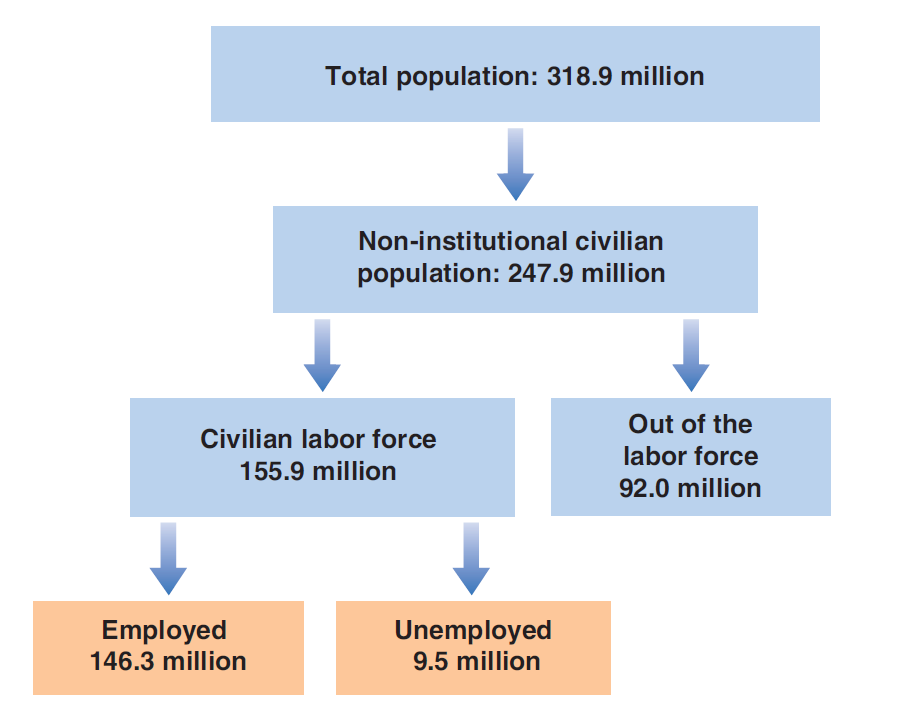
\includegraphics[width=1\textwidth]{7_1} %插入图片,[]中设置图片大小,{}中是图片文件名
	\caption{Population, Labor
		Force, Employment,
		and Unemployment in
		the United States} %最终文档中希望显示的图片标题
	\label{Fig.main2} %用于文内引用的标签
\end{figure}

非公众机构民间人员:除去那些不够工作年龄、在军队服役以及在监狱服刑的人员,潜在的可供民间雇佣的人员。

民间劳动力:正在工作和寻找工作的人。

退出劳动力:要么不在劳动力市场工作,要么放弃了找工作。

参与率(participation):劳动力占非公共机构民间人员的比例。

失业率(unemployment rate):劳动力中失业人员的比例。

官方统计没有把像做饭以及带孩子这样的家务活动视为工作,对这些活动是否是工作作出价值判断很困难。

\subsection{劳动力的大规模流动}

给定的失业率可能反映了两种完全不同的现实。可能是活跃的劳动力市场有许多人离职(separations),也有很多人就职(hires)。也可能是僵化的劳动力市场,很少有人离职也很少有人就职,劳动力大军是停滞的。

离职的人中:一部分从一份工作到另一份工作,一部分人退出劳动力市场,剩下的人从就业变成失业。

离职的人中,有辞职的(quits),劳动者找到了更好的工作而辞掉当前的工作,剩下的是被解雇的(layoffs),解雇往往是因为企业的雇用人员数量发生变化。(离职人数=辞职人数+解雇人数)

平均失业持续时间:每个月摆脱失业的失业人员的比例的倒数。当失业水平高的时候,比如在危机期间,平均失业持续时间也将大大增加。

被归为“退出劳动力市场”的人中有一部分很像失业人员,他们实际上是丧失信心的劳动者(discouraged workers)。虽然他们并没有积极寻找工作,但是找到工作的时候就会接受。

反向考虑:一些失业人员可能不愿意接受提供的工作,也许不应该被归类为失业,因为他们并没有真正寻找工作。

就业率(employment rate),就业人口占可以工作人口的比例。失业水平越高,或者退出劳动力市场的人数越多,就业率越低。

\section{失业的变化}

有时失业率的峰值出现在经济衰退之后,而非经济衰退当年。究其原因,尽管产出为正,从而技术上来讲,经济已经走出了衰退,但是增加的产出并没有增加足够多的就业机会来降低失业率。

\hspace*{\fill}

总失业率的波动在从两个方面影响单个劳动者:

总失业率波动对单个劳动者福利的影响;

总失业率对工资的影响。

如果企业通过减少雇佣新员工来调整雇员人数,那么失业人员找到工作的机会会减少。更少的雇佣意味着更少的招聘机会,更高的失业率意味着更多的求职者。更少的招聘会和更多的求职者使失业者找工作越发麻烦。

如果企业通过多解雇来调整,那么已雇员工失业的风险变高。

一般来说,企业双管齐下,较高失业率既和失业人员面临找到工作的机会变小有关,又和就业人员面临失去工作的风险变高有关。

\hspace*{\fill}

总结一下,当失业率高时,劳动者的情况恶化主要表现在以下两方面:

已就业的劳动者失去工作的可能性变高;

失业劳动者找到工作的可能性变低,也就是说,预期失业将持续更长时间。

\section{工资的决定}

工资的决定有很多决定方式。有时通过集体谈判(collective bargaining),即企业和工会协商来确定。其余的,或者由雇主决定,或者由雇主和单个雇员协商决定。工作所需技能越高,协商的可能性越高。国与国之间差别也很大。

虽然制度的差别会影响工资的决定,但所有国家有一些共同力量在起作用,主要体现在以下两个方面:

劳动者得到的工资往往高于他们的保留工资(reservation wage)。保留工资指的是是人们感觉工作和失业无差异的工资水平。

工资一般取决于劳动力市场的状况。失业率越低,工资越高。

\hspace*{\fill}

经济学家对上述结论的两种解释:

第一,即使没有集体谈判,大多数工人也有一定的协商能力,使他们获得的工资高于保留工资。

第二,企业自身因为各方面的原因,愿意支付高于保留工资的工资。

\subsection{议价}

工人的议价能力(bargaining power)取决于两个因素:一是如果工人离开企业,为了替代该工人企业可能的花费;二是找到另一份工作的难易程度。企业替代工人花费的成本越高,工人找其他工作越容易,那么工人的议价能力就越强。其中包含的两层意思:

工人的议价能力首先取决于工作的性质。

工人的议价能力还取决于劳动力市场的状况。失业率低的时候,企业找到合适的替代者就比较难,同时,工人也比较容易找到其他工作,这种情况下,工人就有比较高的议价能力,也可能获得更高的工资。反之反是。

\subsection{效率工资}

抛开工人的议价能力,企业也许愿意支付比保留工资更高的工资。它们希望工人更有效率,而较高的工资能做到这一点。

还有一个更一般的命题:多数企业希望员工对他们的工作有自豪感,这样能促使他们更好地工作,从而提高工作效率。增加工资只是企业达到这一目的的方法之一。

经济学家把将工人的生产率或效率与工资联系起来的理论称为效率工资理论(efficiency wage theories)。

\hspace*{\fill}

与基于议价的理论类似,效率工资理论说明工资取决于工作的性质和劳动力市场的状况。

企业,比如高科技企业,视员工的士气和担当为工作质量至关重要的部分,也愿意支付比常规部门员工更多的工资。

当失业率低时,容易找到另一份工作,也就是说,企业为了减少员工离职,必须增加工资使他们留下来。当这些发生时,低失业率又会导致新一轮的工资上涨。相反,高失业率会导致低工资。

\subsection{工资、价格和失业}

工资的决定:

\[
W=P^eF(u,z)
\]

名义总工资——W,由三个因素决定:

预期价格水平——$ P^e $;

失业率——u;

其他因素——z,代表可能影响工资的其他变量(跟工资同向变动)。

\subsection{预期价格水平}

为什么价格水平会影响名义工资:这是由于工人和企业都关系实际工资而不是名义工资。

工人们不关心他们得到了多少钱,但关心这些钱能买到多少东西。换句话说,他们不关心得到的名义工资,但关心得到的名义工资W和他们要买的商品价格P之比W/P。

同样企业不关心它们支付的名义工资,而是名义工资W和它们所出售的商品价格P之比W/P。

预期价格水平上升导致名义工资的同比例上升。

由于工资是以名义形式(美元)设定的,在设定的时候,相关价格水平是未知的。因此工资取决于预期价格水平$ P^e $而不是实际价格水平P。

\subsection{失业率}

失业率上升会导致工资降低。

如果我们认为工资取决于议价,那么较高的失业率会削弱工人的议价能力,他们只能接受低工资。如果我们认为工资取决于对效率工资的考虑,那么失业率较高时,企业支付较低的工资仍然能促使工人去工作。

\subsection{其他因素}

z代表在给定预期价格水平和失业率影响下工资的全部其他因素。根据习惯,定义z使z增加时工资也会增加。

其他因素有:失业保险、最低工资、就业保护。

\section{价格的决定}

产品的定价取决于企业面临的成本。这些成本又取决于生产函数的性质。

现在,我们假设企业只使用劳动力这种单一的生产要素来生产产品,那么,生产函数为:

\[
Y=AN
\]

其中,Y是产出,N是就业人数,A是劳动生产率。

进一步假设A=1,生产函数变为:

\[
Y=N
\]

这个生产函数意味着,多生产一单位产出的成本是多雇佣一个工人的成本,即工资W。用微观经济学的术语就是:边际成本——增加一单位产出的成本,等于W。

如果产品市场是完全竞争市场,那么一单位产出的价格就会等于边际成本,即$ P=W $,但很多产品不是竞争性的,企业的定价就会高于边际成本,定义:

\[
P=(1+m)W
\]

其中m是价格超过成本的加成(markup)。如果产品市场是完全竞争的,那么m等于0,价格P超过成本W。当市场不是竞争性的,企业就会获得市场势力,那么m是正的,价格P会超过成本W,乘上一个因子(1+m)。

m反映垄断程度/竞争性的缺乏程度/准入门槛/勒纳指数。


\section{自然失业率}

假设名义工资取决于实际价格水平P而不是预期价格水平$ P^e $,在这个附加假设条件下,工资和价格的设定决定均衡失业水平。

\subsection{工资设定关系}

在名义工资取决于实际价格水平P,而不是预期价格水平$ P^e $的假设条件下:

\[
W=PF(u,z)
\]

在等式两边同时除以价格:

\[
\frac{W}{P}=F(u,z)
\]

工资的决定说明实际工资$ W/P $和失业率之间是负相关的;失业率越高,工资设定者选择的实际工资就越低。把实际工资和失业率之间的关系称为工资设定关系(wage-setting relation)。

\subsection{价格设定关系}

考虑价格决定的影响:

\[
\frac{P}{W}=1+m
\]

两边倒置:

\[
\frac{W}{P}=\frac{1}{1+m}
\]

这个等式的含义为:价格设定决策决定企业支付的实际工资。在一定工资水平下,加成的增加导致价格上涨,同样也会导致实际工资下降。

价格设定关系(price-setting relation)是水平线PS。价格设定导出的实际工资是$ 1/(1+m) $,它不取决于失业率。

\begin{figure}[H] %H为当前位置,!htb为忽略美学标准,htbp为浮动图形
	\centering %图片居中
	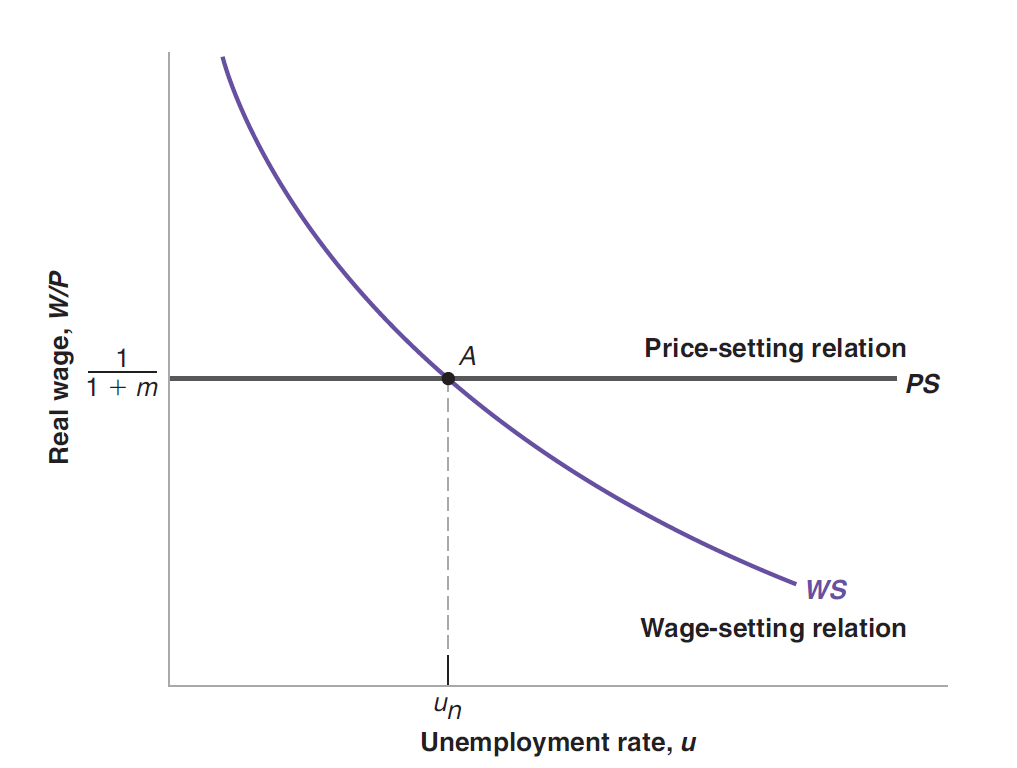
\includegraphics[width=1\textwidth]{7_2} %插入图片,[]中设置图片大小,{}中是图片文件名
	\caption{Wages, Prices, and
		the Natural Rate of
		Unemployment} %最终文档中希望显示的图片标题
	\label{Fig.main3} %用于文内引用的标签
\end{figure}

\subsection{均衡实际工资和失业}

劳动力市场的均衡要求工资设定选择的实际工资等于价格设定导出的实际工资。

用代数的方式描述均衡失业率:

\[
F(u_n,z)=\frac{1}{1+m}
\]

均衡失业率$ u_n $是工资设定选择的实际工资,等于价格设定导出的实际工程时的失业率。这个均衡失业率称为自然失业率(natural rate of unemployment)。

工资设定和价格设定曲线的位置,也就是均衡失业率取决于z和m。

增加失业救济金。增加失业救济金会导致z上升:救济金的增加降低了人们对事业预期的痛苦,在一定的失业率水平下,工资设定者就会提高工资。

总之,在给定的失业率水平下,较高的失业救济金导致较高的实际工资。较高的失业率将实际工资调回到企业愿意支付的水平。

\begin{figure}[H] %H为当前位置,!htb为忽略美学标准,htbp为浮动图形
	\centering %图片居中
	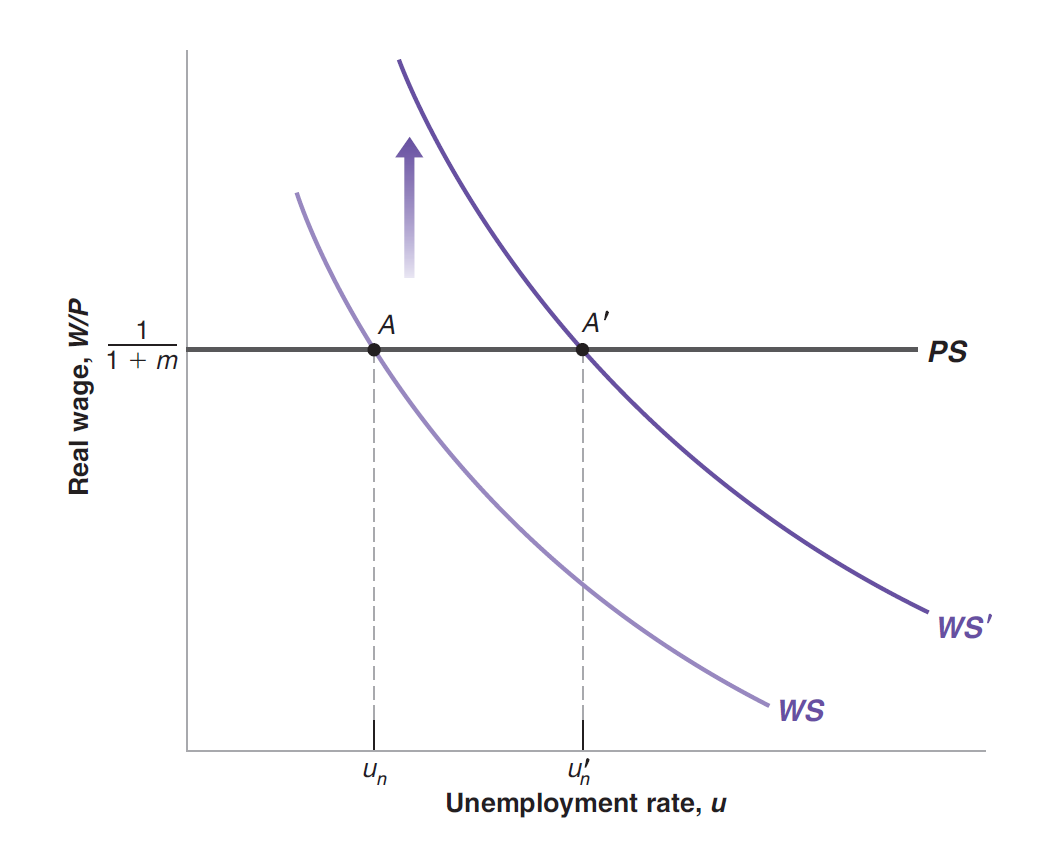
\includegraphics[width=1\textwidth]{7_3} %插入图片,[]中设置图片大小,{}中是图片文件名
	\caption{Unemployment Benefits
		and the Natural Rate of
		Unemployment} %最终文档中希望显示的图片标题
	\label{Fig.main4} %用于文内引用的标签
\end{figure}

弱化反垄断法执行。弱化反垄断法执行在某种程度上使企业串谋更容易,增强了它们的市场势力,也会导致加成上升——m增加。m上升意味着实际工资下降,失业率增加。

在一定工资水平下弱化反垄断法执行,允许企业提高价格,会导致实际工资下降。较高的失业率使工人接受较低的实际工资,从而导致自然失业率上升。

\begin{figure}[H] %H为当前位置,!htb为忽略美学标准,htbp为浮动图形
	\centering %图片居中
	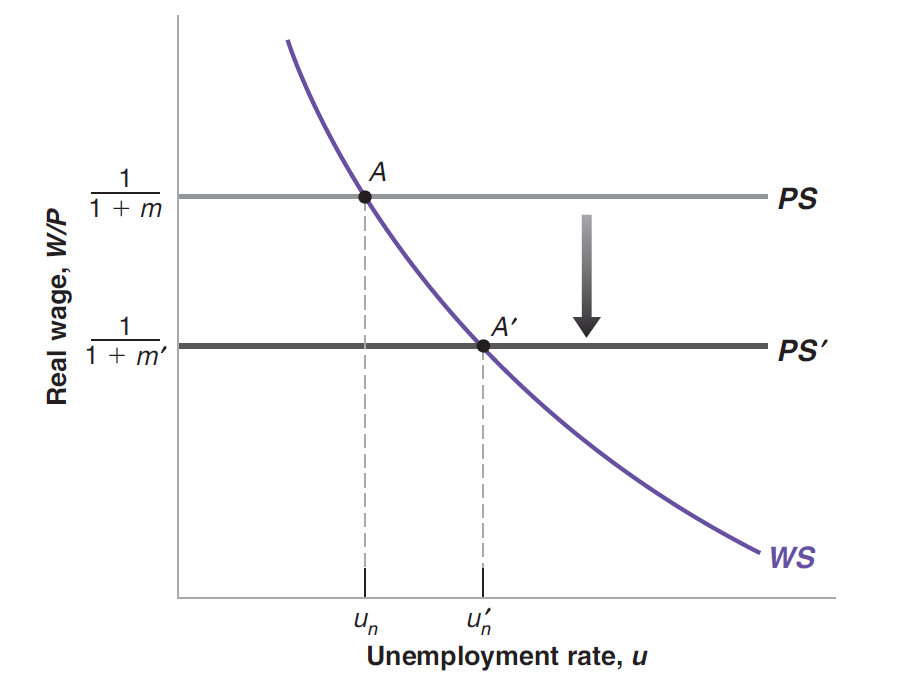
\includegraphics[width=1\textwidth]{7_4} %插入图片,[]中设置图片大小,{}中是图片文件名
	\caption{Markups and the Natural
		Rate of Unemployment} %最终文档中希望显示的图片标题
	\label{Fig.main5} %用于文内引用的标签
\end{figure}

很难认为慷慨的失业救济金和反垄断法是自然作用的结果。相反,它们反映了经济结构的各种特征。基于这个原因,最好把均衡失业率称为结构性失业率(structural rate of unemployment)。

\section{补充}

对给定的劳动力,失业率决定了就业水平;并且,给定生产函数,就业水平决定了产出水平。因此,与自然失业率联系在一起的自然就是自然产出水平。

短期与中期的差异:

我们是在两个假设条件下推出自然失业率和就业与产出之间的联系的。首先,我们假设劳动力市场处于均衡状态。其次,我们假设价格水平等于其预期水平。

但是在短期,没有理由能说明第二个假设条件是正确的。设定工资时,价格水平很有可能不同于预期水平。短期来看,没有理由认为失业率等于其自然水平,或者产出等于其自然水平。

在短期,决定产出变动的因素就是货币政策和财政政策等。

预期不可能一直发生系统性错误(太高或太低),这就是为什么在中期产出会回到自然产出水平。在中期,决定失业和产出的因素是m和z。





\end{document}